\documentclass[border=10pt]{standalone}
\usepackage{tikz}
\usetikzlibrary{arrows.meta, positioning, shapes.geometric, fit, backgrounds, calc}

\definecolor{coreblue}{HTML}{2563EB}
\definecolor{corebluelt}{HTML}{DBEAFE}
\definecolor{topogreen}{HTML}{059669}
\definecolor{topogreenlt}{HTML}{D1FAE5}
\definecolor{agentpurple}{HTML}{7C3AED}
\definecolor{agentpurplelt}{HTML}{EDE9FE}
\definecolor{spicered}{HTML}{DC2626}
\definecolor{spiceredlt}{HTML}{FEE2E2}
\definecolor{programorange}{HTML}{D97706}
\definecolor{programorangelt}{HTML}{FEF3C7}
\definecolor{flowgray}{HTML}{4B5563}
\definecolor{flowgraylt}{HTML}{F3F4F6}

\begin{document}
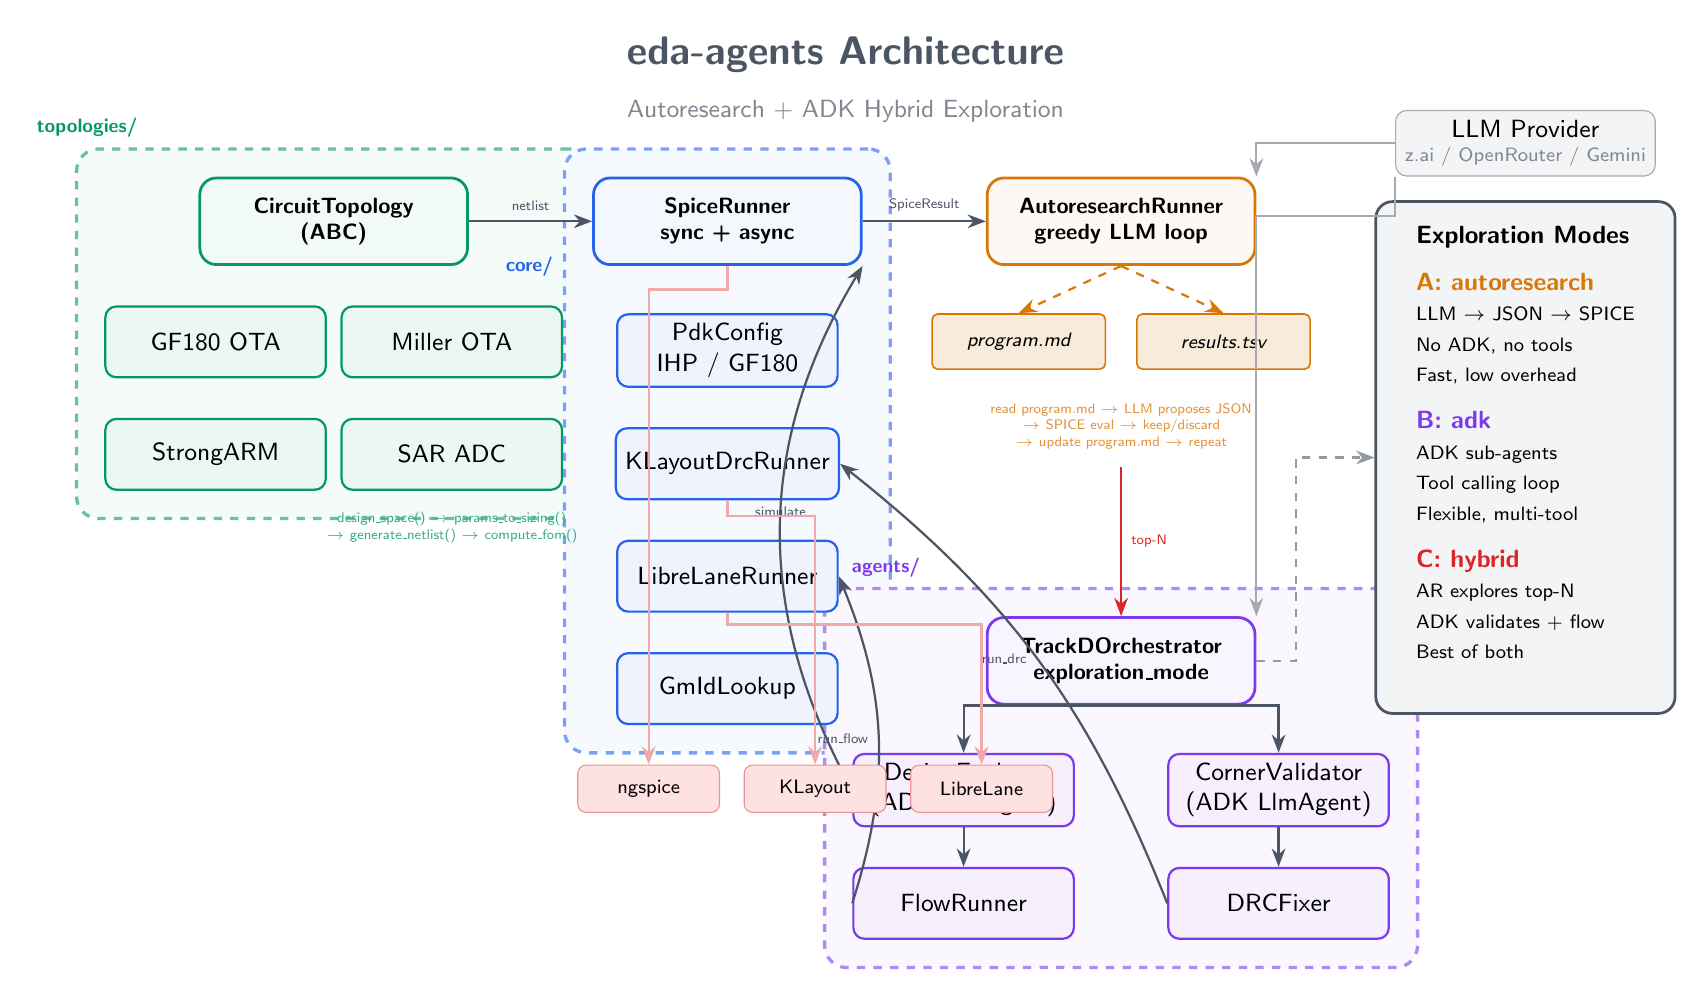
\begin{tikzpicture}[
    >=Stealth,
    node distance=0.8cm and 1.2cm,
    box/.style={
        rectangle, rounded corners=4pt, draw=#1, fill=#1!8,
        minimum width=2.8cm, minimum height=0.9cm,
        font=\sffamily\small, align=center, line width=0.8pt
    },
    bigbox/.style={
        rectangle, rounded corners=6pt, draw=#1, fill=#1!5,
        minimum width=3.4cm, minimum height=1.1cm,
        font=\sffamily\footnotesize\bfseries, align=center, line width=1pt
    },
    filenode/.style={
        rectangle, rounded corners=2pt, draw=#1, fill=#1!15,
        minimum width=2.2cm, minimum height=0.7cm,
        font=\sffamily\scriptsize\itshape, align=center, line width=0.6pt
    },
    groupbox/.style={
        rectangle, rounded corners=8pt, draw=#1!60, fill=#1!4,
        inner sep=10pt, line width=1.2pt, dashed
    },
    arr/.style={->, thick, color=flowgray},
    darr/.style={<->, thick, color=flowgray},
    dataarr/.style={->, thick, color=programorange, dashed},
]

% =====================================================================
% Title
% =====================================================================
\node[font=\sffamily\Large\bfseries, color=flowgray] (title)
    {eda-agents Architecture};
\node[font=\sffamily\small, color=flowgray!70, below=0.1cm of title]
    (subtitle) {Autoresearch + ADK Hybrid Exploration};

% =====================================================================
% Column 1: Circuit Topologies (left)
% =====================================================================
\node[bigbox=topogreen, below=1.2cm of title, xshift=-6.5cm]
    (topo_abc) {CircuitTopology\\(ABC)};

\node[box=topogreen, below=0.5cm of topo_abc, xshift=-1.5cm]
    (gf180) {GF180 OTA};
\node[box=topogreen, below=0.5cm of topo_abc, xshift=1.5cm]
    (miller) {Miller OTA};
\node[box=topogreen, below=0.5cm of gf180]
    (strongarm) {StrongARM};
\node[box=topogreen, below=0.5cm of miller]
    (saradc) {SAR ADC};

% Group
\begin{scope}[on background layer]
\node[groupbox=topogreen, fit=(topo_abc)(gf180)(miller)(strongarm)(saradc),
      label={[font=\sffamily\scriptsize\bfseries, color=topogreen]above left:topologies/}] (topo_group) {};
\end{scope}

% Topology interface
\node[font=\sffamily\tiny, color=topogreen!80, below=0.15cm of saradc, text width=3.2cm, align=center]
    {design\_space() $\to$ params\_to\_sizing()\\$\to$ generate\_netlist() $\to$ compute\_fom()};

% =====================================================================
% Column 2: Core Infrastructure (center-left)
% =====================================================================
\node[bigbox=coreblue, below=1.2cm of title, xshift=-1.5cm]
    (spice) {SpiceRunner\\sync + async};
\node[box=coreblue, below=0.6cm of spice]
    (pdk) {PdkConfig\\IHP / GF180};
\node[box=coreblue, below=0.5cm of pdk]
    (klayout) {KLayoutDrcRunner};
\node[box=coreblue, below=0.5cm of klayout]
    (librelane) {LibreLaneRunner};
\node[box=coreblue, below=0.5cm of librelane]
    (gmid) {GmIdLookup};

\begin{scope}[on background layer]
\node[groupbox=coreblue, fit=(spice)(pdk)(klayout)(librelane)(gmid),
      label={[font=\sffamily\scriptsize\bfseries, color=coreblue]above left:core/}] (core_group) {};
\end{scope}

% =====================================================================
% Column 3: Exploration Modes (center-right)
% =====================================================================

% Autoresearch
\node[bigbox=programorange, below=1.2cm of title, xshift=3.5cm]
    (autoresearch) {AutoresearchRunner\\greedy LLM loop};

\node[filenode=programorange, below=0.6cm of autoresearch, xshift=-1.3cm]
    (program) {program.md};
\node[filenode=programorange, below=0.6cm of autoresearch, xshift=1.3cm]
    (tsv) {results.tsv};

% Autoresearch loop detail
\node[font=\sffamily\tiny, color=programorange!80, below=0.3cm of program,
      text width=4.5cm, align=center, xshift=1.3cm]
    (loop_desc) {read program.md $\to$ LLM proposes JSON\\
     $\to$ SPICE eval $\to$ keep/discard\\
     $\to$ update program.md $\to$ repeat};

% ADK Agents
\node[bigbox=agentpurple, below=2.0cm of loop_desc, xshift=0cm]
    (orchestrator) {TrackDOrchestrator\\exploration\_mode};

\node[box=agentpurple, below=0.6cm of orchestrator, xshift=-2cm]
    (explorer) {DesignExplorer\\(ADK LlmAgent)};
\node[box=agentpurple, below=0.6cm of orchestrator, xshift=2cm]
    (corner) {CornerValidator\\(ADK LlmAgent)};
\node[box=agentpurple, below=0.5cm of explorer]
    (flowagent) {FlowRunner};
\node[box=agentpurple, below=0.5cm of corner]
    (drcfixer) {DRCFixer};

\begin{scope}[on background layer]
\node[groupbox=agentpurple,
      fit=(orchestrator)(explorer)(corner)(flowagent)(drcfixer),
      label={[font=\sffamily\scriptsize\bfseries, color=agentpurple]above left:agents/}] (agent_group) {};
\end{scope}

% =====================================================================
% Column 4: Three Modes (right side, vertical)
% =====================================================================
\node[rectangle, rounded corners=6pt, draw=flowgray, fill=flowgraylt,
      minimum width=3.8cm, minimum height=6.5cm,
      right=1.5cm of autoresearch, yshift=-3cm,
      font=\sffamily\small, align=left, inner sep=8pt, line width=1pt]
    (modes) {
    \textbf{Exploration Modes}\\[6pt]
    \textcolor{programorange}{\textbf{A: autoresearch}}\\
    \scriptsize LLM $\to$ JSON $\to$ SPICE\\
    \scriptsize No ADK, no tools\\
    \scriptsize Fast, low overhead\\[6pt]
    \textcolor{agentpurple}{\textbf{B: adk}}\\
    \scriptsize ADK sub-agents\\
    \scriptsize Tool calling loop\\
    \scriptsize Flexible, multi-tool\\[6pt]
    \textcolor{spicered}{\textbf{C: hybrid}}\\
    \scriptsize AR explores top-N\\
    \scriptsize ADK validates + flow\\
    \scriptsize Best of both\\
    };

% =====================================================================
% Arrows: data flow
% =====================================================================

% Topology -> SpiceRunner (netlist)
\draw[arr] (topo_abc.east) -- node[above, font=\sffamily\tiny, color=flowgray]{netlist} (spice.west);

% SpiceRunner -> Autoresearch
\draw[arr] (spice.east) -- node[above, font=\sffamily\tiny, color=flowgray]{SpiceResult} (autoresearch.west);

% Autoresearch <-> program.md
\draw[dataarr] (autoresearch.south) -- (program.north);
\draw[dataarr] (autoresearch.south) -- (tsv.north);

% Autoresearch -> Orchestrator (top-N in hybrid mode)
\draw[arr, color=spicered] ($(loop_desc.south)+(0,-0.1)$) -- node[right, font=\sffamily\tiny, color=spicered]{top-N} (orchestrator.north);

% Orchestrator -> sub-agents
\draw[arr] (orchestrator.south) -| (explorer.north);
\draw[arr] (orchestrator.south) -| (corner.north);
\draw[arr] (explorer.south) -- (flowagent.north);
\draw[arr] (corner.south) -- (drcfixer.north);

% Sub-agents -> core tools
\draw[arr, bend right=20] (flowagent.west) to node[left, font=\sffamily\tiny]{run\_flow} (librelane.east);
\draw[arr, bend right=15] (drcfixer.west) to node[left, font=\sffamily\tiny]{run\_drc} (klayout.east);

% Explorer -> SpiceRunner
\draw[arr, bend left=30] (explorer.west) to node[above, font=\sffamily\tiny]{simulate} (spice.south east);

% Orchestrator -> modes box
\draw[arr, dashed, color=flowgray!60] (orchestrator.east) -- ++(0.5,0) |- (modes.west);

% =====================================================================
% LLM Provider (top right)
% =====================================================================
\node[rectangle, rounded corners=4pt, draw=flowgray!50, fill=flowgraylt,
      minimum width=2.6cm, minimum height=0.8cm,
      above=0.3cm of modes, font=\sffamily\small, align=center]
    (llm) {LLM Provider\\[-2pt]\scriptsize\color{flowgray!70} z.ai / OpenRouter / Gemini};

\draw[arr, color=flowgray!50] (llm.west) -| (autoresearch.north east);
\draw[arr, color=flowgray!50] (llm.south west) -- ++(0,-0.5) -| (orchestrator.north east);

% =====================================================================
% External tools (bottom)
% =====================================================================
\node[rectangle, rounded corners=3pt, draw=spicered!50, fill=spiceredlt,
      minimum width=1.8cm, minimum height=0.6cm,
      below=0.5cm of gmid, xshift=-1cm, font=\sffamily\scriptsize]
    (ngspice) {ngspice};
\node[rectangle, rounded corners=3pt, draw=spicered!50, fill=spiceredlt,
      minimum width=1.8cm, minimum height=0.6cm,
      right=0.3cm of ngspice, font=\sffamily\scriptsize]
    (klayout_ext) {KLayout};
\node[rectangle, rounded corners=3pt, draw=spicered!50, fill=spiceredlt,
      minimum width=1.8cm, minimum height=0.6cm,
      right=0.3cm of klayout_ext, font=\sffamily\scriptsize]
    (librelane_ext) {LibreLane};

\draw[arr, color=spicered!40] (spice.south) -- ++(0,-0.3) -| (ngspice.north);
\draw[arr, color=spicered!40] (klayout.south) -- ++(0,-0.2) -| (klayout_ext.north);
\draw[arr, color=spicered!40] (librelane.south) -- ++(0,-0.15) -| (librelane_ext.north);

\end{tikzpicture}
\end{document}
